\section*{Proof for IO Integrity}
\label{appendix:security}

In this appendix, we provide a formal proof of the following property: \emph{without protecting both input and output integrity, none of them can be achieved}. 


\subsection{Interaction Protocol} 
\label{appendix:security:protocol}

To simplify the proof, we model the interaction between the user, the host, and the remote server as a finite state automaton (FSA).
The interactions between the server (\server), the user (\user) and host (\host) are depicted in the FSA in Figure~\ref{fig:fsm}.

\begin{figure}[h!]
\begin{center}
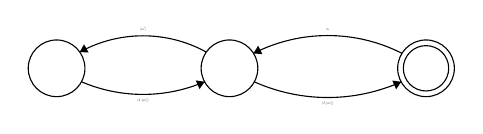
\begin{tikzpicture}[scale=0.15]
\tikzstyle{every node}+=[inner sep=0pt]
\draw [black] (66,-23.1) circle (3);
\draw (66,-23.1) node {\server};
\draw [black] (66,-23.1) circle (2.4);
\draw [black] (45.2,-23.1) circle (3);
\draw (45.2,-23.1) node {\host};
\draw [black] (26.9,-23.1) circle (3);
\draw (26.9,-23.1) node {\user};
\draw [black] (47.743,-21.516) arc (116.95563:63.04437:17.332);
\fill [black] (47.74,-21.52) -- (48.68,-21.6) -- (48.23,-20.71);
\draw (55.6,-19.13) node [above] {$m$};
\draw [black] (29.352,-21.382) arc (118.8302:61.1698:13.89);
\fill [black] (29.35,-21.38) -- (30.29,-21.43) -- (29.81,-20.56);
\draw (36.05,-19.16) node [above] {$[m']$};
\draw [black] (42.565,-24.526) arc (-66.78269:-113.21731:16.527);
\fill [black] (42.57,-24.53) -- (41.63,-24.38) -- (42.03,-25.3);
\draw (36.05,-26.36) node [below] {$(I,[m'])$};
\draw [black] (63.369,-24.535) arc (-65.91058:-114.08942:19.034);
\fill [black] (63.37,-24.53) -- (62.43,-24.4) -- (62.84,-25.32);
\draw (55.6,-26.69) node [below] {$(I,[m'])$};
\end{tikzpicture}
\end{center}
\caption{Finite state machine that depicts the interaction between the user (\user), host (\host) and the server (\server).}
\label{fig:fsm}
\end{figure}

\server sends a message $m$ to \host. One can assume $m$ to be the HTML, JavaScript, and other data send from \server as a HTTP response. We denote $[m]$ to be the render of $m$ by the \host. As \host is malicious, it can transform $m$ to $m'$. Note that the transformation is public knowledge and is deterministic. If $m\neq m'$ then given $[m]$ and $[m']$, \server can determine that $[m]\neq [m']$. We denote the user input to be $I$, which corresponds to a specific $[m]$. 
%Note that the communication channel between \server to \user is neither authenticated, neither confidential. But the communication channel from \user and \server is authenticated. 
In this model, we simplify the user input by assuming that the \user only provides an input $I$ only after observing a message transformation $[m]$. The user provides both her input $I$ and transformation $[m']$ observed by her to \host. The interaction loop between \host and \user can continue until \user finishes her input. After every input \host hands over new message transformation to \user (either result of the input or new message from \server or both). Once the user provides all her inputs, \host send the pairs $(I, [m'])$ to \server.

We also define two mappings:
\begin{align*}
\texttt{Input()}&:[m]\rightarrow I \\
\texttt{Transform()}&:m,I\rightarrow [m'],\ \exists i\in I:i=\phi
\end{align*}
Both of them are \emph{bijective}.

One trace of the protocol transcript is depicted in Figure~\ref{fig:protocol}. As described in the FSM, \server receives traces of message transformation ($[m']_1,[m']_2,\ldots,[m']_n$) and corresponding inputs ($I_1,I_2,\ldots,I_n$). From these traces \server could determine of all the $[m']_i$ are in proper form by verifying if $[m]_i=[m']_i$.

\begin{figure}[t]
\begin{center}
\tikzset{
  every picture/.append style={
    transform shape,
    scale=0.8
  }
 }
\begin{sequencediagram}
\newinst{u}{\user}
\newinst[3]{h}{\host}
\newinst[3]{s}{\server}
\mess{s}{$m$}{h}
\mess{h}{$[m']_1$}{u}
\mess{u}{$I_1,[m']_1$}{h}
%\mess{h}{$[m']_2$}{u}
%\mess{u}{$I_2,[m']_2$}{h}
\mess{h}{...}{u}
\mess{u}{...}{h}
\mess{h}{$[m']_n$}{u}
\mess{u}{$I_n,[m']_n$}{h}
\mess{h}{$I_1,I_2,...,I_n$}{s}
\mess{h}{$[m']_1,[m']_2,...,[m']_n$}{s}
\end{sequencediagram}
\end{center}
\caption{Protocol transcript between the \server, \user and \host that shows one trace from the FSM depicted in Figure~\ref{fig:fsm}.}
\label{fig:protocol}
\end{figure}


\begin{definition}{\textbf{Input integrity}}
\label{def:inputIntegrity}
Assume that \server handed a message $m$ to \host where the proper message transformation is $[m]$. The host changes the message transformation to $[m']$ where $[m']\neq [m]$. We also define correct \user input to be $I$ when \host sends a correct message transformation $[m]$ to \user. We define input integrity as the property where the \server does not accept input $I'$ where $I'\neq I$from \user if the \host changes the message transformation.
\end{definition}

\begin{definition}{\textbf{Output integrity}}
\label{def:outputIntegrity}
Assume that \server handed a message $m$ to \host where the proper message transformation is $[m]$. Output integrity defines that in all circumstances, \user receives the correct message transformation $[m]$ from \host.
\end{definition}

\myparagraph{Verification process} \server checks $\forall i=1\ldots n$ $$[m']_i = \texttt{Transform}(m_{i-1}, I_{i-1})$$ where $I_0=\phi$.

\begin{theorem}
\label{theorem:th1}
If \user does not send all the transformations till $[m']_i$ corresponding to the input $I_i$, input integrity can not be achieved. 
\end{theorem}

\begin{IEEEproof}
If \user does not attach all the transformation till $[m']_i$, i.e., $[m']_1, [m']_2, \ldots, [m']_{i-1}, [m']_i$  corresponding to inputs $I_1, I_2,\ldots, I_{i-1}, I_i$, then the server can not verify all the transformations corresponding to the input. \host could modify a specific $[m]_x$ to influence \user input.
\end{IEEEproof}

\begin{theorem}
\label{theorem:th2}
If the channel from \user and \server is not authenticated, input integrity is not achievable. But the channel from \server to \user does not require to be secure as long a \user provides the message transformation $[m']_i$ corresponding to every input $I_i$.
\end{theorem}

\begin{IEEEproof}
The proof is trivial. If the channel from \user to \server is not authenticated, any input provided by \user can be manipulated by \host without a trace. Hence input integrity is not achievable. As long as \user sends message transformation along with the input, a manipulated message transformation bt \host would be detectable by \server (see Theorem~\ref{theorem:th1}).
\end{IEEEproof}

\begin{theorem}
\label{theorem:th3}
Ensuring output integrity also ensures input integrity provided there is an authenticated channel from \user to \server.
\end{theorem}

\begin{IEEEproof}
This proof is also trivial. As we describe in the Definition~\ref{def:inputIntegrity} and~\ref{def:outputIntegrity}, if all the message transform from \host $[m']=[m]$, and \host always executes \texttt{transform()} properly, the input integrity is preserved. As \name ensures output integrity and all the input from the user is signed by the \device, \name preserves input integrity. 
\end{IEEEproof}


\section*{Implementation Details}
\label{appendix:implementation}

\subsection{HID Drivers}


\red{We use Arduino prototype development board as the HID drivers. Figure~\ref{fig:prototype} shows an Arduino Due, and a Zero board where the Due connects to the HIDs via the native USB port and the Zero relays the HID data to the Raspberry Pi (RPi). The Due and the Zero boards are connected over $I^2C$ interface. As both Due and Zero only have one native USB port on each of them, we were forced to use two boards as an HID interceptor and relay. The Zero relays the HID signals both to the connected host (over native USB) and to the RPi (over serial interface). The connection from the Zero to the host is one way and emulates a composite HID. While the connection between the Zero and the RPi is bidirectional. The HID drivers are implemented using the native Arduino \texttt{keyboard} and \texttt{mouse} library. On the RPi, no HID drivers were needed as the RPi receives processed HID data from the Zero (for the pointer: displacement over x and y-axis and for keyboard, ASCII characters).}

\subsection{HDMI Interceptor, Relay and Overlay}

\red{The RPi along with the Auvidea B101 HDMI to CSI bridge, acts as the HDMI interceptor and relay. The B101 board converts HDMI signals from the host as a camera input (via the CSI interface) to the RPi. This allows the RPi to access the HDMI frames as a stream of JPEG frames. The HDMI out of the RPi acts as the relay that connects to the monitor. On the RPi, we use Picamera API~\cite{picamera} to access the HDMI frames. The B101 is capable of processing 25 frames at 1080p resolution. Hence, this is the hardware bottleneck of our implementation. However, the upcoming B112 board\footnote{still in development: \url{https://auvidea.eu/showcase/}.} could solve this performance issue.
On the RPi, the overlay and HDMI out is implemented using Java SWT. Using SWT, we create a full-screen window that is shown on the monitor. The SWT class polls the HDMI frames and process them as individual JPEG images via the \texttt{BufferedImage} class. This allows the overlays to be drawn on the HDMI images efficiently. The Java program uses a QR code interpreter to extract the UI specification. Based on the UI specification, it creates the geometrical shapes (corresponding to the UI elements) and draw them on the frames. In the current implementation of the \name, the UI elements such as button, text-field, radio button etc. are preloaded in the \device memory. Note that the current implementation of \device is based on the RPi. But one could implement such functionality on an FPGA, reducing the TCB even more. 
}

\subsection{Mouse Pointer Tracking}

\begin{figure}[h]
\centering
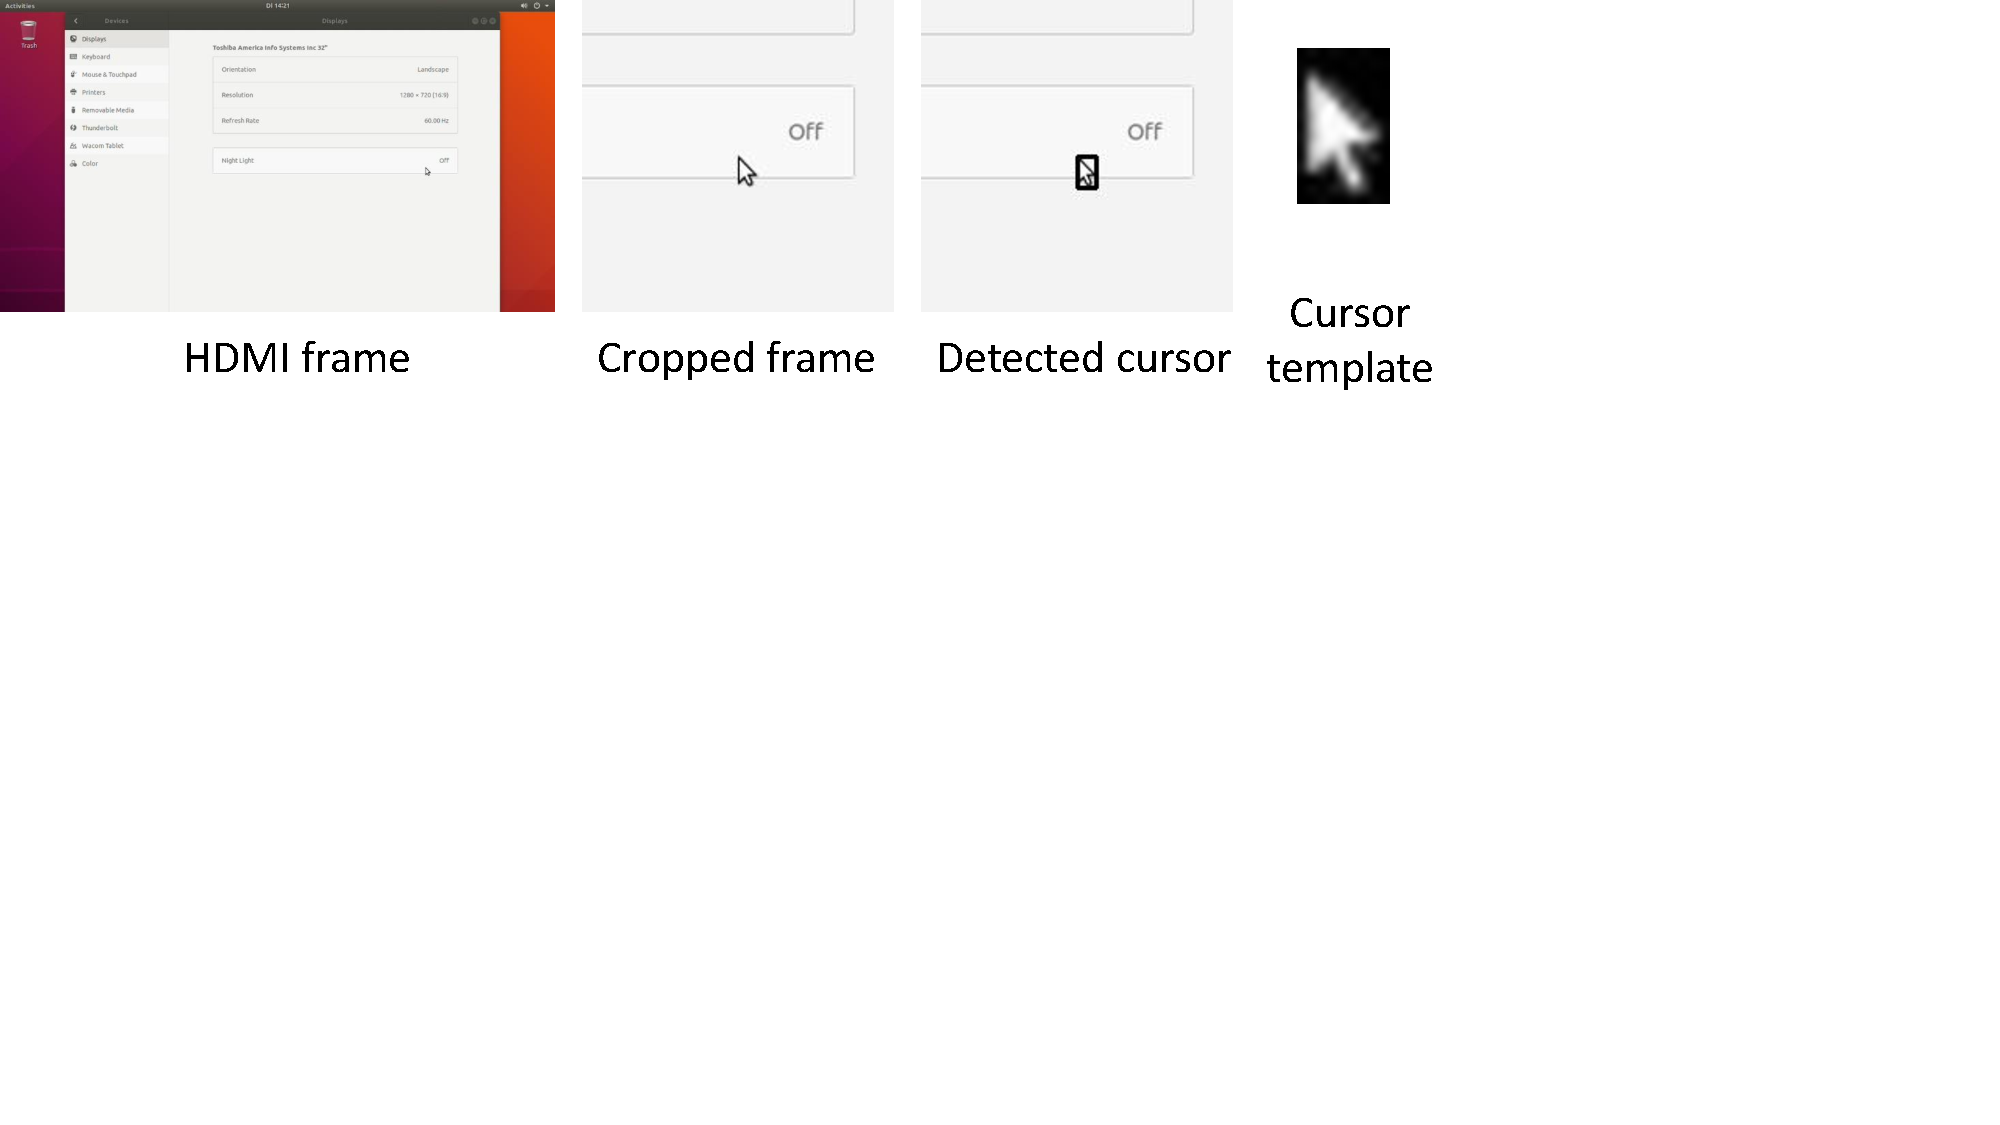
\includegraphics[trim={0 12cm 10cm 0}, clip, width=\linewidth]{cursorDetect.pdf}
\caption{\textbf{Cursor detection on the HDMI frame.} .}
\spacesave
\label{fig:cursorDetect}
\centering
\end{figure} 

\red{The pointer tracing is also executed in the aforementioned Java program using simple object detection technique suppled by the OpenCV API. Figure~\ref{fig:cursorDetect} shows one screenshot of the pointer detection. The Figure shows the entire HDMI frame, the cropped frame (based on the mouse input data), the detected pointer in the cropped frame and the cursor template that is used by the object detection algorithm.
}


